\documentclass[MASTER.tex]{subfiles}
\begin{document}
%============================================================%


%================================================================== %
\begin{frame}
\frametitle{Zero-Truncated Poisson regression}
\large
\textbf{Data Set :  hospitalstay}
\begin{itemize}
	\item 
We have a hypothetical data file, \textbf{\textit{hospitalstay}} with 1,493 observations. 
\item The length of hospital stay variable is \textbf{stay}. 
\item The variable \textbf{age} gives the age group from 1 to 9 which will be treated as interval in this example. 
\item The variables \textbf{hmo} and \textbf{died} are binary indicator variables for HMO insured patients and patients who died while in the hospital, respectively.
\end{itemize}
\end{frame}
%========================================================== %
\begin{frame}[fragile]
\frametitle{Zero-Truncated Poisson regression}
\textbf{Data Set :  hospitalstay}
\begin{verbatim}
##       stay            age       hmo      died   
##  Min.   : 1.00   Min.   :1.00   0:1254   0:981  
##  1st Qu.: 4.00   1st Qu.:4.00   1: 239   1:512  
##  Median : 8.00   Median :5.00                   
##  Mean   : 9.73   Mean   :5.23                   
##  3rd Qu.:13.00   3rd Qu.:6.00                   
##  Max.   :74.00   Max.   :9.00
\end{verbatim}
\end{frame}
%=========================================================== %
\begin{frame}
\begin{figure}
\centering
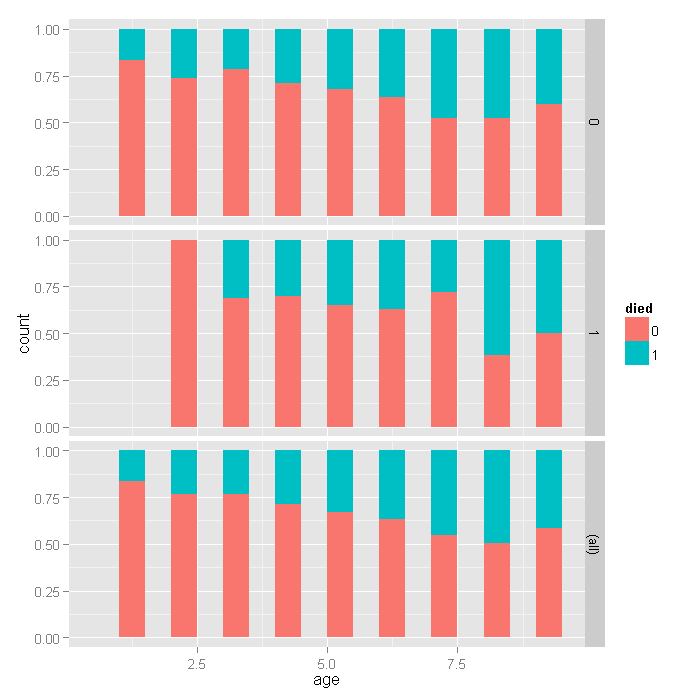
\includegraphics[width=0.8\linewidth]{hospitalstay}

\end{figure}
\end{frame}
%=========================================================== %
\begin{frame}
\frametitle{Zero-Truncated Poisson regression}
\large
\textbf{Data Set :  hospitalstay}
	\begin{itemize}
\item For the lowest ages, a smaller proportion of people in HMOs died, but for higher ages, there does not seem to be a huge difference, with a slightly higher proportion in HMOs dying if anything. \item Overall, as age group increases, the proportion of those dying increases, as expected.
	\end{itemize}

	
	
\end{frame}



\end{document}